\clearpage{\pagestyle{empty}\cleardoublepage}
\chapter{Il datacenter}\label{sec:datacenter}
Il datacenter \`e il componente del sistema responsabile della elaborazione 
del flusso informativo generato dai dispositivi \emph{di campo} installati 
presso i vari impianti sotto monitoraggio.
%
Si tratta di un sistema software costituito da diverse applicazioni, ciascuna 
delle quali implementa una o pi\`u delle funzionalit\`a tra quelle riportate di seguito:
%
\begin{itemize}
  \item decodifica dei \emph{dati di campo}
  \item stima di grandezze \emph{aggregate}
  \item memorizzazione dei dati su \emph{memoria persistente}
  \item rilevamento di \emph{condizioni anomale} e generazione di \emph{allarmi}
  \item fornire accesso allo \emph{stato} degli impianti
  \item fornire accesso ai \emph{dati storici} degli impianti
\end{itemize}
%

%
Dall'elenco delle funzionalit\`a, \`e facile osservare come il
datacenter ricopra un ruolo fondamentale all'interno del sistema di monitoraggio: 
si tratta di un componente \emph{critico}, un suo malfunzionamento 
(ad esempio uno \emph{shutdown} dovuto a un \emph{crash}) puo` avere effetti che 
vanno dalla semplice interruzione del servizio di accesso ai dati degli impianti 
fino alla mancata decodifica dei dati provenienti dai dispositivi di campo e, 
quindi, al blocco \emph{de facto} dell'intero sistema di monitoraggio.
%
Per questo motivo, durante la prima fase della progettazione, sono stati 
individuati, oltre ai gi\`a elencati requisiti funzionali, un insieme di 
\emph{propriet\`a} di cui il datacenter avrebbe dovuto godere. Tali propriet\`a 
sono:
%
\begin{itemize}
\item \emph{liveness}, i.e. una volta verificatosi un evento di interesse, 
il datacenter deve, prima o poi, gestirlo; tale propriet\`a serve a garantire, ad 
esempio, che ogni \emph{batch} di dati provenienti dai dati di campo venga, 
presto o tardi, processato.
%
\item \emph{high availability}, i.e. il datacenter deve essere costantemente 
in esecuzione, salvo \emph{downtime} programmati per operazioni quali 
aggiornamento release, etc.
%
\item \emph{robustness}, i.e. l'esecuzione del datacenter non deve essere 
compromessa da situazioni anomale quali, ad esempio, la ricezione di dati 
\emph{malformati} da parte di dispositivi di campo in avaria. Il datacenter 
deve essere in grado di rilevare potenziali anomalie.%% e segnalarle?
%
\item \emph{scalability}, i.e. le prestazioni del datacenter non devono 
decrescere all'aumentare del numero di impianti, e, quindi del numero di 
flussi informativi, da monitorare. %% e se un giorno volessi distribuire il datacenter?
%
\end{itemize}
%% dire due parole sul fatto che sono proprieta` note?
%

%
Tali propriet\`a hanno fortemente condizionato il successivo \emph{step} di
progettazione, ovvero la scelta della \emph{tecnologia} su cui costruire il 
datacenter, che \`e, infine, ricaduta su Erlang/OTP.
%

%
Questo capitolo \`e organizzato come segue: il prossimi due paragrafi
introdurranno Erlang/OTP e si soffermeranno sui motivi che ne fanno la scelta %% e introduranno dei concetti fondamentali per descrivere il sistema
tecnologica pi\`u adatta. Successivamente, a partire dal paragrafo 
\ref{datacenter-arch} verr\`a descritta l'architettura del datacenter.
%

%
\section{Breve introduzione a Erlang/OTP}%%
OTP \`e l'acronimo di \emph{Open Telecom Platform}. Rilasciato da \emph{Ericsson} 
a partire dal 1998, si tratta di un \emph{middleware} per applicazioni distribuite 
scritte in Erlang\cite{erlang}. Il suo campo di applicazione, a dispetto di quanto 
il nome possa lasciar intendere, va ben oltre le telecomunicazioni.
%

%
Una definizione pi\`u articolata di cosa sia OTP \`e fornita da Joe Armstrong in 
\cite{armstrong07}: \emph{OTP is an application operating system and a set of libraries 
and procedures used for building large-scale, fault-tolerant, distributed applications}.
%

%
\subsection{Behaviours}
%
L'intera architettura di OTP si basa sul concetto, fondamentale, di \emph{behaviour}:
un behaviour \`e un componente astratto che implementa un determinato 
\emph{design pattern} tipico della \emph{programmazione concorrente}, p.es. il modello di 
interazione \emph{client/server}. 
%
I behaviour OTP, nel loro complesso, forniscono \emph{a set of standardized building 
blocks used in designing and building industrial-grade systems}\cite{cesarini09}.
%
In altre parole, citando \cite{armstrong07}, il loro utilizzo consente agli sviluppatori 
di concentrarsi sulla parte \emph{funzionale} dell'applicazione, i.e. la \emph{business logic}, 
lasciando che il middleware si occupi di gestire gli aspetti \emph{non funzionali}, quali 
\emph{fault-tolerance}, \emph{scalability}, \emph{dynamic code upgrade}, ecc.
%

%
I behaviour e i moduli application-specific vanno poi collegati, al fine di definire 
un processo Erlang, mediante l'implementazione di opportune \emph{callback}.
%
\begin{figure}[!h]
\centering
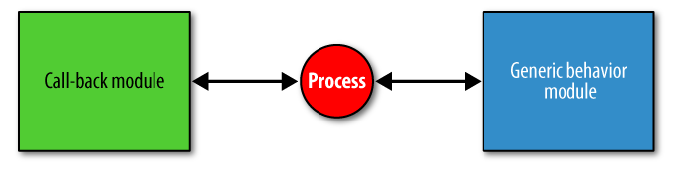
\includegraphics[width=400pt]{img/erl-behaviour.png}
\caption{Processo Erlang costituito da un behaviour e da un modulo di callback}
\end{figure}
%

%
\subsection{Supervision Tree}
%
Esistono due particolari classi di behaviours: \emph{worker} e \emph{supervisor}\cite{otpsupervisor}; 
%
i primi rappresentano i processi che si occupano di effettuare \emph{concretamente} del lavoro, 
p.es. \emph{servers}, \emph{event handlers}, \emph{finite state machines}, ecc.
%
i secondi, invece, si occupano di supervisionare i propri \emph{figli}, i quali possono essere sia
worker che, a loro volta, dei supervisors. 
%
Tra le responsabilit\`a di un supervisor vi sono:
\begin{itemize}
\item \emph{avviare} i processi i figli
\item (opzionalmente) \emph{riavviare} i processi figli in caso di \emph{fault}
\item \emph{terminare} i processi figli al termine dell'applicazione
\end{itemize}
%

%
Il \emph{supervision tree} non \`e altro che una rappresentazione delle relazioni di supervisione 
all'interno di un sistema basato su OTP.
%
\begin{figure}[!h]
\centering
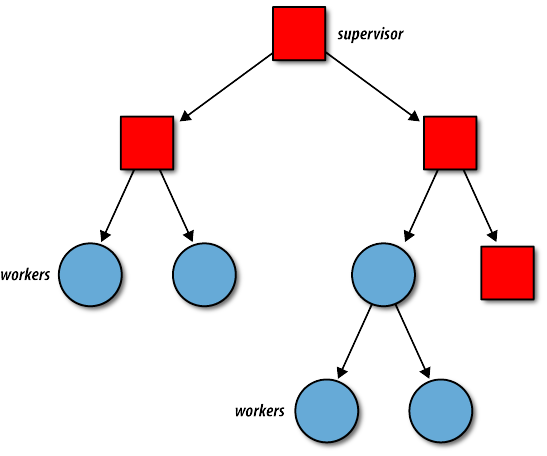
\includegraphics[width=350pt]{img/supervision-tree.png}
\caption{Esempio di supervision tree}
\end{figure}
%

%

%
\subsection{Applications}
%
I supervision tree costituiscono, in un certo senso, lo \emph{scheletro} di ogni applicazione
basata su OTP. Esiste, infatti, un behaviour detto \emph{application}\cite{otpapplication}, 
il cui ruolo \`e quello di raggruppare un insieme di supervision trees, rendendoli 
\emph{riusabili}. 
%

%
In generale, una applicazione OTP \emph{is a reusable component that packages library modules 
together with supervisor and worker processes}\cite{cesarini09}.

%
Una sistema basato su OTP \`e, quindi, formato da un insieme di \emph{application} distribuite 
e lascamente accoppiate, ciascuna delle quali implementa una determinata funzionlit\`a.
%
%% supporto per erlang applications: restart, etc.

%
\section{Perch\`e OTP}
%% bit syntax














%% architettura: insieme di erlang applications:
\section{L'architettura del datacenter}
\label{datacenter-arch}
\section{L'applicazione \emph{sysconf}}
%
\begin{figure}[!h]
\centering
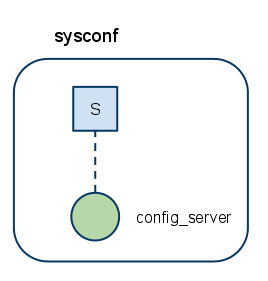
\includegraphics[width=180pt]{img/sysconf.png}
\caption{Supervision tree dell'applicazione Sysconf}
\end{figure}
%
\section{L'applicazione \emph{datamanager}}
%
\begin{figure}[!h]
\centering
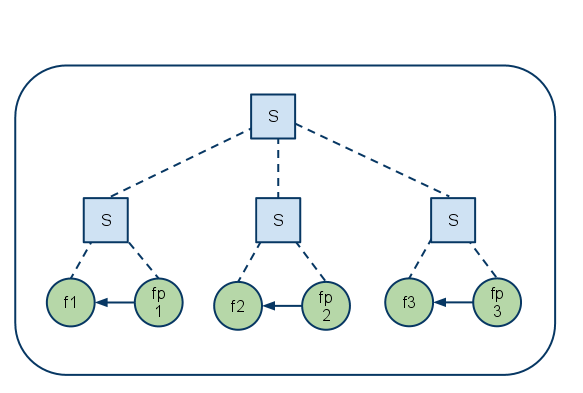
\includegraphics[width=380pt]{img/datamanager.png}
\caption{Supervision tree dell'applicazione Datamanager}
\end{figure}
%
\subsection{Il filter}
\subsection{Il file\_poller}
%
\begin{figure}[!h]
\centering
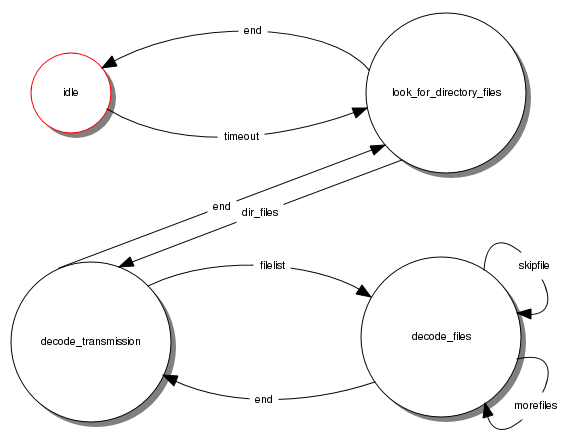
\includegraphics[width=300pt]{img/file-poller.png}
\caption{Sequenza di polling}
\end{figure}
%
\subsection{La decodifica: \emph{ftp\_protocol}}
%% il supervision tree
\section{L'applicazione \emph{database}}
%
\begin{figure}[!h]
\centering
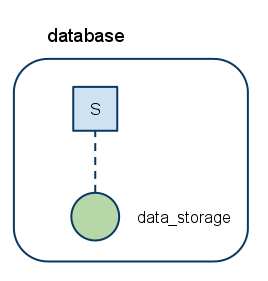
\includegraphics[width=180pt]{img/database.png}
\caption{Supervision tree dell'applicazione Database}
\end{figure}
%
\cite{erl-amnesia}
\section{L'applicazione \emph{datamanager-ws}}
